\documentclass[useAMS,usenatbib,referee,12pt]{article}
\usepackage[margin=1.0in]{geometry}
\usepackage{amsmath}
\usepackage{amssymb}
\usepackage{amsfonts}
\usepackage{parskip}
\usepackage[round]{natbib}
\usepackage{color}
\usepackage[dvipsnames]{xcolor}
\usepackage{caption}
\usepackage{tabularx, booktabs}
\usepackage{float}
\usepackage{adjustbox}
\usepackage[toc,page]{appendix}
\usepackage{enumitem}
\usepackage{multirow}
\usepackage{setspace}
\doublespacing

\newcommand{\adam}[1]{{\color{blue} ADAM: #1}}
\newcommand{\jarad}[1]{{\color{Orange} #1}}
\newenvironment{indpar}[1]%
     {\begin{list}{}%
             {\setlength{\leftmargin}{#1}}%
             \item[]%
     }
     {\end{list}}

\newcommand{\vn}{\textbf{n}}

\begin{document}

%\tableofcontents 

\begin{abstract}

Abundance estimates from animal point-count surveys require accurate estimates of detection probabilities.  
The standard model for estimating detection from removal-sampled point-count surveys assumes that organisms at a survey site are detected at a constant rate; however, this assumption is often not justified.  
Detection rates can be influenced by organismal behaviors, survey methodology, and observer effort.  
Failure to account for non-constant detection leads to biased estimates of detection and therefore of abundance.  
Whereas, under the standard approach, detection probability is modeled by dividing the observation period into equal-duration intervals, we instead model the detection {\it rate} in continuous time via a time-to-detection distribution embedded within a hierarchical N-mixture framework using Bayesian methods.  
Our model is thus a combination of survival time-to-event analysis with unknown-N, unknown-p abundance estimation.  
We apply this model to Ovenbird counts from the Chippewa National Forest and to datasets simulated under different time-to-detection patterns.  
Models assuming constant detection rates produce biased estimates of detection when true detection rates vary with time, whereas models allowing for variable detection (assuming gamma, Weibull, or lognormal distributed times to detection) produce less biased estimates of the detection probability and nominal credible interval coverage.  
Models ignoring detection heterogeneity across subgroups yield biased estimates of detection when such heterogeneity exists, whereas models accounting for detection heterogeneity (modeled as a mixture) return reasonable coverage rates and can outperform heterogeneity-ignorant models even when there is no heterogeneity.

{\bf Keywords:} abundance; availability; N-mixture model; survival analysis; Bayesian

\end{abstract}

\section{Introduction}\label{sec:intro}

\adam{WRITE A SPELLBINDING OPENING PARAGRAPH}\jarad{no need to aim so high}

%Farnsworth's removal assumptions:\\
%(i) Closed population during survey\\
%(ii) no double-counting\\
%(iii) easy-to-detect group is entirely counted during first interval\\
%(iv) TTDD for hard-to-detect group is correct after the end of the observation period\\
%(v) if using limited radius counts, they are accurate
% Johnson2008: all birds present are available for detection

Removal sampling is a species abundance surveying methodology in which observers capture and physically remove animals at a survey site over a series of trapping sessions.  
Assuming that the probability of capturing a not-yet-trapped individual is the same for all trapping sessions, it is possible to estimate the proportion of individuals still not captured from the pattern of captures over time \citep{Moran1951, Zippin1958, Seber1982}.  
\citet{Farnsworth2002} adapted removal sampling to avian point-count surveys, suggesting that observers record just the first time-to-detection for each bird and mentally remove it thereafter.  
Analysis proceeds by subdividing the observation period into intervals of equal duration and assuming that the rate of detection is the same at all times (i.e., following a Poisson process); then, each interval can be treated as a trapping event, and the interval-specific probability of detection can be estimated as with conventional removal sampling.

However, the assumption of a constant detection rate throughout the observation period is not always justified \citep{Alldredge2007}.  
Animal behaviors such as bout singing or intermittent singing in birds and frogs or diving in whales can lead to time-varying rates of detection \citep{Scott2005, Diefenbach2007, Reidy2011}.  
The act of observation may affect animal behavior.  
Depending upon the study species, the presence of an observer may temporarily either stimulate or suppress detectable cues \citep{McSheaRappole1997, Rosenstock2002, Alldredge2007}.  
Survey methodology itself can affect detection rates.  
Observers may also become distracted as the survey progresses \citep{Johnson2008}.  
And, depending upon protocol, observers may become aware of animals during their settling-in period, resulting in elevated counts early during in the survey period \citep{LeeMarsden2008}.  
In the presence of detection heterogeneity, easily detected animals will be removed first, leaving only harder to detect animals, thus resulting in a marginal detection rate that varies over time \citep{Farnsworth2005}.

In this study, we develop a model for scenarios where detection rates are not constant.  
We model time-to-detection as is done in survival analysis, defining a continuous random variable $T$ for each animal's time to first detection with a probability density function (pdf) $f_T(t)$ and cumulative distribution function $F_T(t)$.  
We refer to the distribution of $T$ as a time-to-detection distribution (TTDD).  
The instantaneous detection rate or hazard function $h(t)$ can be found from the TTDD as $h(t) = f_T(t) / (1-F_T(t))$.

Unlike most survival analyses, the number of individuals $N$ present at a survey is unknown.  
We embed the TTDD in a hierarchical framework for multinomial counts using an N-mixture model \citep{Wyatt2002, Royle2004NMixture}.  
For our purposes, the N-mixture framework provides three clear benefits.  
First, its multinomial data framework accords with the interval censored data collection that is customary in point-count surveys \citep{Ralph1995}.  
Second, the hierarchical structure readily lends itself to including abundance- and detection-related covariates and random effects \citep{Dorazio2005, Etterson2009, Amundson2014}.  
Third, for a Bayesian analysis, we can sample the posterior joint distribution of N-mixture parameters straight-forwardly using Markov chain Monte Carlo (MCMC).  
The N-mixture framework models abundance as a latent variable with a Poisson or other discrete distribution and independently models detection probabilities.  
Several previous studies have employed the N-mixture framework to analyze removal sampled point-count data while assuming constant detection rates \citep{Royle2004Generalized, Dorazio2005, Etterson2009, Solymos2013, Amundson2014}.  


Framing a model in terms of time-to-detection leads to two practical differences vis-a-vis constant-detection models.  
First, in order to model covariate and random effects on detection, we perform mixed effects linear regression on the log of the rate parameter as in \citet{Solymos2013}, whereas most existing studies instead construct regression models on the logit of the equal-interval detection probability \adam{Amundson2014 and others?}.  
Such an approach is not possible when detection rates are not constant.  
Second, because we can obtain interval-specific detection probabilities from the TTDD by partitioning its cdf, we can directly model the data according to their existing interval structure rather than subdividing the observation period into intervals of equal duration.  
Indeed, with a few simplifications, our model fits exact time-to-detection data, whereas existing constant-detection removal models only approximate exact data by subdividing the observation interval into a large number of fine intervals \citep{Reidy2011, Amundson2014}.

\adam{Based on further lit review, I think I need to insert a paragraph here about what time-varying modeling has been done.  
In the fisheries world, models of time-varying catchability have been implemented -- see Schnute 1983, Scruton and Gibson (ref: Mantyniemi), and Mantyniemi2015 for examples.  
Also, Alldredge 2007 implements a complete-history of detection model (technically mark-recapture, not removal) that estimates interval-specific detection probabilities (complete with covariates and detection heterogeneity).  
However, it cannot be applied in a removal context, because removal data contains only first times to detection, and the Alldredge model requires subsequent observations -- removal models compensate by specifying a TTDD, thus enabling us to extrapolate beyond the observation period.}  

\jarad{The introduction needs to end earlier. It should be about 1-2 pages covering what has previously been done and outline our approach. So this should probably start a new section and before this there should be an outline of our manuscript. }

\subsection{TTDDs as behavior and methodology}

A TTDD defines the range of detection patterns possible in an analysis.  
The most basic is an exponential TTDD, which imposes a constant first detection rate.  
Choosing another TTDD can allow for a systematic non-constant detection regime.  
For example, to model an observer effect where: (i) the observer's arrival suppresses or stimulates detectable cues, but (ii) organisms acclimate and gradually return to constant detection, a gamma TTDD could be appropriate (Figure \ref{HazardFxns}).

Increasing hazard functions result in a pdf for $T$ that has a mode away from zero; we term these TTDDs `peaked'.  
We contrast these to decreasing hazard functions with a mode at zero, which we term `non-peaked'.  
For our purposes, the exponential TTDD is neither peaked nor non-peaked.

We distinguish between non-constant detection and detection heterogeneity, which can be modeled in similar ways but refer to different mechanisms.  
We reserve `detection heterogeneity' for differences across population subgroups.  
It is often modeled using a mixture of detection distributions.  
\citet{Farnsworth2002} introduce a partial finite-mixture for detection probabilities distinguishing between easy-to-detect individuals, which are always detected in first observation interval, and hard-to-detect individuals, which are detected at a constant rate.  
 Heterogeneity at the individual level can be modeled as random effects in the calculation of detection probabilities \citep{DorazioRoyle2003, Mantyniemi2005}.  
We use `non-constant detection' when detection rates for an organism change with time.  
Models constructed to address detection heterogeneity may provide reasonable estimates for non-constant detection scenarios and vice versa \citep{Mantyniemi2005}.

\adam{Individual effects on detection might suffer from identifiability issues. This was the subject of a dust-up between Pledger and Dorazio/Royle from 2003-2005.}

\begin{figure}[h!]\centering
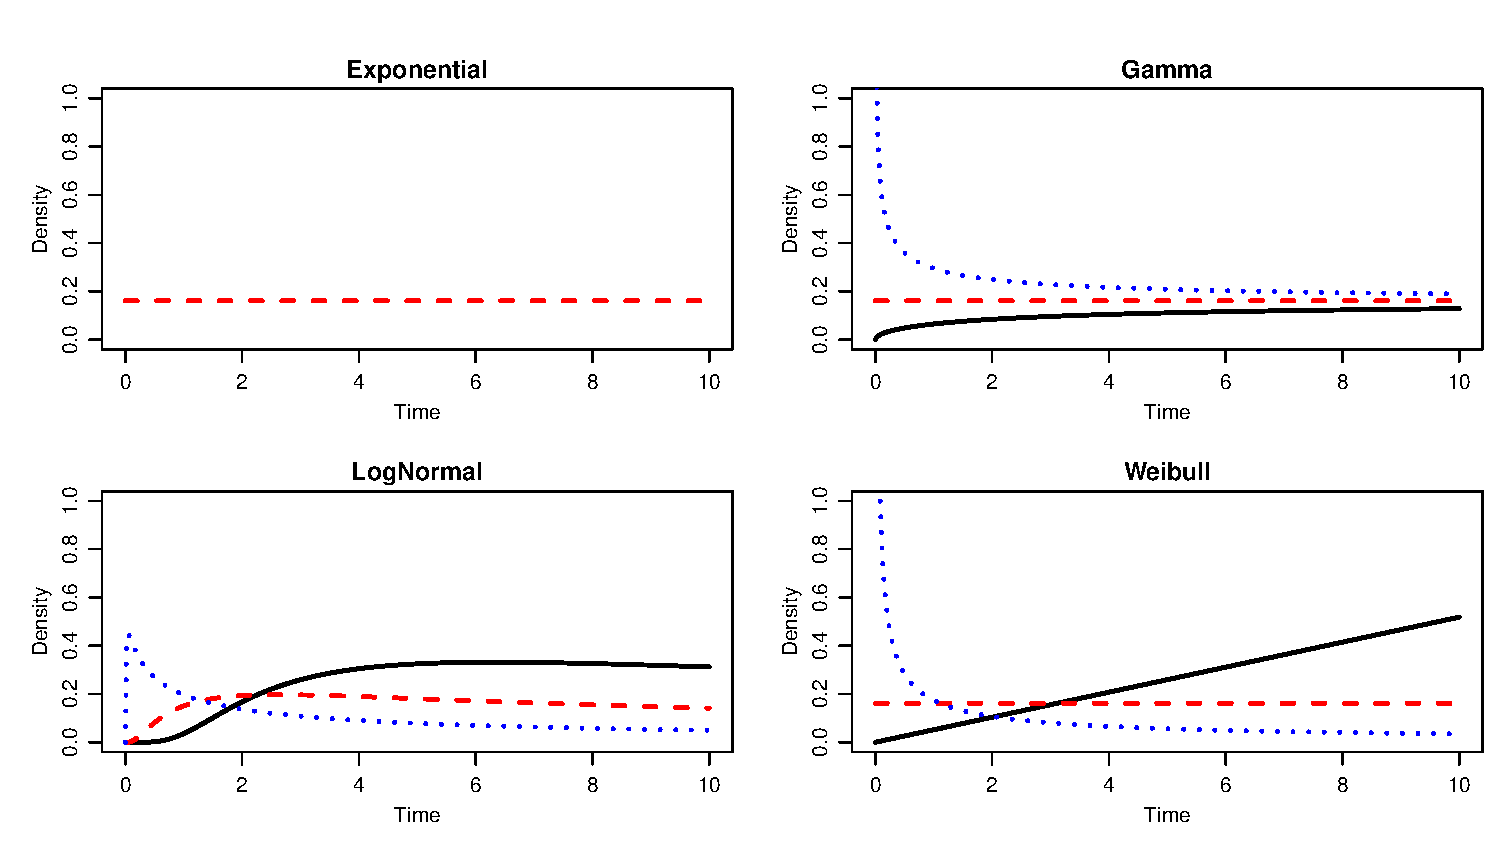
\includegraphics[width=0.68\textwidth]{Hazards}
\caption{Examples of instantaneous rates of detection (hazard functions) from exponential, gamma, lognormal, and Weibull TTDDs.}
\label{HazardFxns}
\end{figure}

In this study, we construct a time-to-detection N-mixture model for estimating abundance from removal-sampled point-count surveys.  
We explore model behavior through a series of simulations testing: (i) how well constant-detection models fit non-constant detection data and vice versa, (ii) the utility of a partial finite-mixtures to model detection heterogeneity involving a non-constant detection subgroup, and (iii) model performance with covariates and random effects affecting both abundance and detection.  
Finally, we apply our model to Ovenbird data from the Minnesota Forest Breeding Bird Project.




\section{Methods}\label{sec:model}

\subsection{Data}\label{sec:data}

Our analysis is motivated by point-count surveys conducted in Chippewa National Forest over a six-year period from 2008-2013 as part of the Minnesota Forest Breeding Bird Project (MNFB).  
The MNFB design is described in \citet{Hanowski1995}, and we summarize only essential details here.  
Single-visit time-to-first-detection point-count surveys are conducted by trained observers at a fixed set of sampling locations once annually.  
Survey durations are 10 minutes, with times to first detection for over 50 species being censored into nine intervals -- a two-minute interval followed by eight one-minute intervals.  
The relatively fine-scale interval sizes should provide more information about TTDDs than the three-interval methodology (0-3, 3-5, and 5-10 minutes) that characterizes many avian point count surveys \citep{Ralph1995}.
There is no prescribed settling-in period between the observer's arrival and the time they begin observing.  

Our model is formulated for single-visit removal-sampled point-count surveys $s=1,\dotso,S$.  
We present the model for exact time-to-detection data and also show how to modify it for interval-censored detection times.  
We use $n_{s}^{(obs)}$ to denote the number of individuals observed during a survey.  
For exact data, times to detection are $t_{sq}$, where $q = 1,\dotso,n_{s}^{(obs)}$ indexes observed individuals at a survey.  
For interval-censored data, we enumerate the intervals $i = 1,\dotso,I$ with the cutoff times for each interval written $C_i$, where $C_0 = 0 \text{ and } C_I = \text{the survey duration}$.  
The number of animals counted during any interval is $n_{si}$, the vector of counts for a survey is written $\vn_{s}$, and $n_{s}^{(obs)} = \sum_{i=1}^I n_{si}$.

\subsection{Framework}

We construct a hierarchical model of removal-sampled point-counts in three pieces: (a) a data model incorporating binomial detection and time-to-detection pieces, (b) a detection model based upon a TTDD, and (c) an abundance model based upon an integer-valued distribution.  
Our model incorporates covariates and random effects for both abundance and detection via mixed effects linear regression.

\subsection{Data Model}
We assume that counts from different surveys are conditionally independent.  
We define $T_{sq}$ as a random variable for the first time at which an individual is detected.
We assume that detection times for individuals at any given survey are independent, identically distributed according to a TTDD with cdf $F_T(t)$ and pdf $f_T(t)$, which may depend on covariates.  
The probability of detecting an animal is thus $p_{s}^{(det)} = Pr(t_{sq} < C_I) = F_T(C_I)$ and the conditional distribution of observed detection times can be written $f_{T|det}(t|t_{sq}<C_I) = f_T(t) / F_T(C_I)$.  
Given $N_{s}$ total number animals present at a survey, the data model is:
\begin{align}\label{eq:datamodel}
n_{s}^{(obs)} &\sim \mbox{Binomial}\left(N_{s}, p_{s}^{(det)}\right)\\
\label{eq:Tsrq}T_{sq} &\sim f_{T|det}(t|t_{sq}<C_I)
\end{align}
When detection times are censored, we replace Eq. \ref{eq:Tsrq} with $\vn_{s} \sim \mbox{Multinomial}\left(n_{s}^{(obs)}, \textbf{p}_{s}\right)$, where $\textbf{p}_{s}$ is the vector of interval-specific detection probabilities obtained by partitioning the conditional cdf $F_{T|det}(t|t_{sq}<C_I)$ at the interval cutoff times.  
It follows that $\sum_{i=1}^I p_{si} = 1$.



\subsection{Detection Model}\label{sec:detectionmodel}

The two main elements of the detection model for $T_{sq}$ are: (i) the distributional form and (ii) the expectation function.
$T_{sq}$ should be based on non-negative continuous distributions featuring some variety of rate parameter than can be estimated via regression.  
In this study, we adopt TTDDs for $T_{sq}$ using the following: Exponential($\varphi_{s}$), Gamma($\alpha, \varphi_{s}$), Weibull($k, \varphi_{s}$), and Lognormal($\mu_{s}, \sigma_{det}^2$).  
Here, $\varphi_{s}$ and $\mu_{s}$ are survey-specific detection rate parameters, and we consider the shape parameters $\alpha$, $\sigma_{det}^2$, and $k$ to be constant across all surveys.

We can model detection heterogeneity by defining $T_{sq}$ as a mixture of TTDD components.  
In this study, we use interval-censored observations, so in addition to the four above TTDDs (with no mixture component), we consider partial finite-mixtures of a point mass during the first survey interval plus a component from an exponential, gamma, Weibull, or lognormal distribution.  
We define a constant mixing parameter $\gamma \in [0,1]$ for the proportion of animals not distributed according to the point mass.

We model the expectation function via mixed effects linear regression.  
For exponential, gamma, and Weibull TTDDs, we model the log of the rate parameter $\varphi_{s}$.  
In so doing, we equivalently model the log of the expected time-to-detection, which is inversely related to the detection rate.  
For the lognormal distribution, we fit a regression to $-\mu_{s}$.  
%Thus, the link functions in our detection model are:
%\begin{alignat}{3}
%&\text{Exponential:\;} &&\log(\varphi_{s}) &&= \text{Intercept}^D + \textbf{X}_{s}^D\boldsymbol{\beta}^D + \textbf{Z}_{s}^D\boldsymbol{\xi}^D = -\log(E[T_{sq}])\\
%&\text{Gamma:} &&\log(\varphi_{s}) &&= \text{Intercept}^D + \textbf{X}_{s}^D\boldsymbol{\beta}^D + \textbf{Z}_{s}^D\boldsymbol{\xi}^D = -\log(E[T_{sq}]) + \log(\alpha)\\
%&\text{Weibull:}  &&\log(\varphi_{s}) &&= \text{Intercept}^D + \textbf{X}_{s}^D\boldsymbol{\beta}^D + \textbf{Z}_{s}^D\boldsymbol{\xi}^D = -\log(E[T_{sq}]) + \log\left(\Gamma\left(1 + 1/k\right)\right)\\
%&\text{Lognormal:} &&-\mu_{s} &&= \text{Intercept}^D + \textbf{X}_{s}^D\boldsymbol{\beta}^D + \textbf{Z}_{s}^D\boldsymbol{\xi}^D = -\log(E[T_{sq}]) + \sigma_{det}^2/2
%\end{alignat}

Combining the distribution and expectation function for $T_{s}$, we can describe a partial-mixture TTDD cdf as:
\[F_T(t|\textbf{X}_{s}^D, \textbf{Z}_{s}^D, \boldsymbol{\theta}) = (1-\gamma)\mathbb{I}(t>0) + \gamma F_{T1}(t|\textbf{X}_{s}^D, \textbf{Z}_{s}^D, \boldsymbol{\theta})\]
where: $F_{T1}$ is the cdf of the non-point-mass component, $\textbf{X}_{sr}^D$ are covariates, $\boldsymbol{\beta}^D$ is a vector of fixed effects, $\textbf{Z}_{sr}^D$ specify random effect levels, $\xi_i^D \overset{ind}{\sim} N(0,\sigma_{D[i]}^2)$ are random effects, with $\sigma_{D[i]}^2$ denoting the variance associated with $\xi_i^D$, and $\boldsymbol{\theta}$ is a vector of parameters appropriate to the TTDD being used.  
$F_T(t|\cdot)$ becomes a non-mixture TTDD if we fix $\gamma=1$.
Note that parameters in a mixture TTDD do not share the exact same interpretation as equivalent parameters from a non-mixture TTDD, since they only pertain to the $\gamma$ proportion of individuals that follow $F_{T1}$.




\subsection{Abundance Model}

For simplicity, we model total abundance at each survey $N_{s}$ using a Poisson distribution, though any non-negative integer-valued distribution may be used.  
We model the expected survey abundance $\lambda_{s}$ via mixed effects linear regression with a log link: $\log (\lambda_{s}) = \textbf{X}_{s}^A\boldsymbol{\beta}^A + \textbf{Z}_{s}^A\boldsymbol{\xi}^A$.  As with the detection model, $\textbf{X}_{sr}^A$ are covariates, $\boldsymbol{\beta}^A$ is a vector of fixed effects, $\textbf{Z}_{sr}^A$ specify random effect levels, and $\xi_i^A \overset{ind}{\sim} N(0,\sigma_{A[i]}^2)$ are random effects.  
We can decompose $N_{s}$ into observed and unobserved portions; the latent unobserved portion follows a binomial-Poisson hierarchy, with the result that $n_{s}^{(unobs)} \sim \mbox{Poisson}\left(\lambda_{s}(1-p_{s}^{(det)})\right)$.  




\subsection{Ovenbird analysis}\label{sec:ovenbirdanalysis}
To demonstrate our model, we fit counts of Ovenbirds (\textit{Seiurus aurocapilla}) from the MNFB.
We restricted survey sites in our analysis to those of the most abundant habitat type (sawtimber red pine); in so doing, we focused modeling efforts upon the detection model and skirted the complication of modeling abundance across habitat types.  
We further constrained analysis to 65 sites with a site origin year between 1870-1970.  
In total, we used 381 site-year surveys in our analysis with a total of 947 Ovenbirds counted and a maximum of eight birds counted in any single survey.

For the abundance half of our model, we used four covariates plus two random effects.  
The covariates were: (a) site age, (b) survey year, (c) an indicator of whether the site stock density is over 70\%, and (d) an indicator of whether the site experienced select-/partial-cut logging during the 1990s.  
We associated random effects with each survey year and each stand, with most stands consisting of three survey sites.  
For the detection half of our model, we used covariates for: (a) Julian date, (b) time of day, (c) temperature, (d) an indicator of whether it is the observer's first year in the database, and (e) an interaction between (a) and (d) to approximate a new observer's learning curve \citep{Alldredge2007}.  
69\% of surveys in our dataset involved observers in their first year at MNFB.  
Preliminary model fits did not support the inclusion of quadratic terms for any detection covariates.  
We associated random effects with each observer.  
We centered and standardized all continuous covariates prior to fitting models.

% Effects: * - means signif
% Observer variation - Farnsworth2002, LinkSauer98, LinkSauer97, Dief07 cites Sauer94 & Dief03, Simons et al03
% First-year observer - LinkSauer98
% Time of day - Farnsworth2002, Soly13*, Amundson
% Season (jdate) - Farnsworth2002, Soly13*, Amundson, Dief07
% Quadratic effects - Soly13
% Tree cover (density) - Soly13
% Year (on detection!) - Reidy11, see also Norvell03
% See Table 1 of Johnson2008, see McShea and Rappole, lit review from Warren2013, Rosenstock02





\subsection{Model fitting}\adam{Looking at other papers, the following all tend to get bundled into the same paragraph or two.  It should follow presentation of our data and of our simulation scheme.}

We fit the models by MCMC sampling in the Bayesian statistical software Stan, implemented via the R package \texttt{rstan} version 2.8.0 \citep{Rstan2015}.  
For intercept-only simulations, we instantiated a single chain running 60,000 iterations; for the Ovenbird analysis and simulations with covariates, chains were 250,000-375,000 iterations.  
We discarded half of the iterations as warmup and then thinned by 1 in 10.  
We monitored convergence of the MCMC chains using Geweke diagnostics \citep{Geweke1991}.  
We reran models if the effective sample size for any parameter was below 1000.  
For most models, we accepted Stan defaults for dispersed initial values; however, gamma and Weibull models sometimes failed unless we specified initial values, which we supplied from true parameter values when known or from the posterior means of preliminary short-run models.

We selected priors to be non-informative within a reasonable range of values.  
Normal priors for the detection model intercept term, Intercept$^D$, were chosen so that, based on an intercept-only non-mixture model with scale parameter of 1: (i) median detection probability was $p_{s}^{(det)} = 0.50$, and (ii) 95\% of the prior detection probability was within $p_{s}^{(det)} \in (0.01, 1.0)$.  
Normal priors for Intercept$^A$ centered at a median abundance of 3 birds per site and a 95\% probability of 0-14 birds present (counted and uncounted).  
Because covariates were centered and scaled to mean zero and variance one, normal priors for effect parameters were centered at zero with standard deviations matching the appropriate intercept term.  
For all shape and variance parameters, we chose half-Cauchy(0,1) priors, and for the mixing parameter $\gamma$ we chose a Uniform(0,1) prior.  
All priors were independent.

To assess goodness of fit, we relied on posterior predictive checks \citep{Gelman1996}.  
Posterior predictive checks assess whether a fitted model can effectively replicate datasets that look like the original data in key aspects, which are measured by check statistics.  
In particular, we are concerned with the goodness of fit for the TTDD distribution, so we defined a check statistic for each observation interval:
\[D(n_i) = \sum\limits_{s} n_{si} \big/ \sum\limits_{si} n_{si}\]
which is the proportion of the total count that occurs during interval $i$ marginally across all surveys.  
The posterior predictive p-value associated with each $D(n_i)$ is the proportion of replicate check statistics that have a larger value than the check statistic for the actual data.  
We simulated replicate datasets and calculated the check statistic at each iteration of our MCMC sampling.  
Posterior predictive p-values near to 0 or 1 are potentially indicators of a misspecified model.

We focus inference on the overall detection probability across all surveys: $p^{(det)} = \sum\limits_{s}n_{s}^{(obs)}\big/$ $\sum\limits_{s}N_{s}$.  
Within simulation studies, we compared model estimates to true $p^{(det)}$ values by percent coverage and by posterior p-values --- the proportion of MCMC samples having a smaller value than the true value.  

We compared different models by means of their goodness of fit and deviance information criterion (DIC) \citep{Spiegelhalter2002}.  
For the full model with random effects, which is a missing data model, we used formulation DIC$_7$ from \citet{Celeux2006} for its ease of computation, but we acknowledge that it suffers some difficulties \citep{Celeux2006, Li2014}.





\section{Simulation studies}

\jarad{Not really Jarad's comment.  But he left notes that there should be a separate Sim section with results bundled within it.}

We conduct three simulation studies to assess: (Sim 1) the importance of modeling detection heterogeneity via a partial finite-mixture component, (Sim 2) the impact of misspecifying the TTDD family (e.g., fitting an exponential TTDD model to data generated from a Weibull TTDD), and (Sim 3) model performance in a more complete scenario when both data generation and model fitting include covariates and random effects for abundance and detection.  
Because model behavior may differ between datasets with peaked and non-peaked TTDDs, we simulate both kinds of dataset for gamma, Weibull, and lognormal models.  
For all families, we simulate both mixture and non-mixture datasets.  
In total, we simulate 14 different dataset types.  
Counts are censored into nine-intervals as with the Ovenbird dataset.

In the first simulation study (Sim 1), for all 14 dataset types, we fit models with both mixture and non-mixture TTDD where the family is correctly specified.  
In Sim 2, we consider only mixture TTDD datasets, and we fit them with mixture TTDD models from all four families.  
For both Sim 1 and Sim 2, we simulate and model 16 replicates.  
In Sim 3, we repeat both the first two studies, but: (i) we include covariates and random effects described in Section \ref{sec:ovenbirdanalysis}, and (ii) we perform only a single replicate, because each gamma model takes an average of 5 days to fit.

For the first two simulation studies, we choose true parameter values so that: (i) the expected detection probability is 0.80, (ii) the expected count is the same as observed in the Ovenbird dataset, (iii) when there is a mixture component, we set $\gamma = 0.65$, meaning that 35\% of individuals are immediately detected, (iv) in non-peaked models, 70\% of \textit{detected} individuals are observed during the first two minutes, and (v) in peaked models, the detection mode for `hard to detect' individuals occurs at 5 minutes.  
For Sim 3, we set true parameter values for each dataset equal to the median posterior values obtained when fitting the same TTDD model to the Ovenbird data.  
Since all models applied to the Ovenbird data resulted in non-peaked model fits, we simulated peaked dataset variants by: (i) starting with posterior median Ovenbird estimates, (ii) setting the mixing parameter to $\gamma = 0.65$, and (iii) scaling the Intercept$^D$ and $\sigma_D^2$ terms by 0.25 and 1.1, which on average results in peak detection near 5 minutes and 75-85\% detection across all sites.  
Covariates and random effect levels are taken directly from the Ovenbird dataset.  
Unlike Sims 1 \& 2, overall detection probabilities in Sim 3 are not the same for each dataset.





\subsection{Mixture vs. non-mixture TTDD}\label{sec:mixture}

In the first simulation study, we simulated intercept-only datasets from 14 TTDDs and fit each with both the correctly specified model and one that was correct except for the mixture component (Table \ref{tbl:sim1}).  
When data derive from a mixture model, then inference models that lack a mixture component misestimate the detection probability $p^{(det)}$ badly in every case.  
This is particularly egregious when datasets feature peaked mixtures; then model coverage is always negligible.  
Conversely, when data derive from a non-mixture model, then inference models that include a mixture component perform just as well as the true model.  
Indeed, for non-peaked non-mixture data, the mixture inference model provides more accurate posterior estimates of $p^{(det)}$ than the non-mixture inference model.  
The one exception is the exponential case, where both models estimate $p^{(det)}$ accurately, but the mixture inference model yields credible intervals about 25\% wider than those from its mixture counterpart.

% Possible other comments
%(1) For non-peaked data, the true inference model is biased low\\
%(2) Mixture inference models generate higher estimates than non-mixture models\\
%(3) True models are generally good\\
%(4) Estimates of non-mixture peaked data are much more precise\\
%(5) Note that plots of TTDD at the median are indistinguishable from the truth except in the blatant fail scenario

\begin{table}[ht]\centering\small
\begin{tabular}{l|l|l|l|cccc|cccc||c}
 \multicolumn{4}{c|}{ } & \multicolumn{4}{c|}{\underline{Non-mixture model}} & \multicolumn{4}{c||}{\underline{Mixture model}} & \\
 \multicolumn{4}{c|}{ } & Med. $p$ & Q($p$) & 50\% & 90\% & Med. $p$ & Q($p$) & 50\% & 90\% & $\Delta$ DIC \\ 
  \hline
  \hline
 \parbox[t]{2mm}{\multirow{14}{*}{\rotatebox[origin=c]{90}{TTDD used to simulate data}}} & \parbox[t]{2mm}{\multirow{7}{*}{\rotatebox[origin=c]{90}{Non-mixture}}} & \parbox[t]{2mm}{\multirow{3}{*}{\rotatebox[origin=c]{90}{Nonpk.}}} & Gamma & 0.76 & 0.41 & 0.75 & 0.88 & 0.84 & 0.66 & 0.56 & 0.94 & 0.24 \\ 
 & & &   Lognormal & 0.66 & 0.17 & 0.31 & 0.62 & 0.78 & 0.48 & 0.62 & 1.00 & -0.67 \\ 
 & & &   Weibull & 0.69 & 0.25 & 0.38 & 0.75 & 0.79 & 0.51 & 0.75 & 1.00 & 0.37 \\ 
  \cline{3-13}
 & & &   Exponential & 0.80 & 0.54 & 0.44 & 0.94 & 0.79 & 0.38 & 0.31 & 0.88 & 1.48 \\ 
  \cline{3-13}
 & & \parbox[t]{2mm}{\multirow{3}{*}{\rotatebox[origin=c]{90}{Peaked}}} &  Gamma & 0.80 & 0.55 & 0.50 & 1.00 & 0.82 & 0.70 & 0.38 & 0.88 & 0.96 \\ 
 & & &   Lognormal & 0.78 & 0.31 & 0.50 & 0.94 & 0.80 & 0.48 & 0.62 & 1.00 & 0.97 \\ 
 & & &   Weibull & 0.79 & 0.49 & 0.56 & 0.94 & 0.82 & 0.66 & 0.44 & 0.88 & 1.28 \\ 
  \cline{2-13}
& \parbox[t]{2mm}{\multirow{7}{*}{\rotatebox[origin=c]{90}{Mixture}}} & \parbox[t]{2mm}{\multirow{3}{*}{\rotatebox[origin=c]{90}{Nonpk.}}} & Gamma & 0.67 & 0.17 & 0.12 & 0.81 & 0.76 & 0.41 & 0.69 & 1.00 & 0.51 \\ 
 & & &   Lognormal & 0.56 & 0.04 & 0.00 & 0.31 & 0.72 & 0.30 & 0.44 & 0.88 & 0.33 \\ 
 & & &   Weibull & 0.51 & 0.02 & 0.00 & 0.06 & 0.71 & 0.32 & 0.44 & 1.00 & 2.40 \\ 
  \cline{3-13}
 & & &   Exponential & 0.96 & 1.00 & 0.00 & 0.00 & 0.77 & 0.37 & 0.38 & 0.94 & 122.81 \\ 
  \cline{3-13}
 & & \parbox[t]{2mm}{\multirow{3}{*}{\rotatebox[origin=c]{90}{Peaked}}} & Gamma & 0.28 & 0.00 & 0.00 & 0.00 & 0.74 & 0.33 & 0.31 & 0.88 & 31.84 \\ 
 & & &   Lognormal & 0.22 & 0.00 & 0.00 & 0.00 & 0.76 & 0.36 & 0.38 & 0.94 & 63.65 \\ 
 & & &   Weibull & 0.22 & 0.00 & 0.00 & 0.00 & 0.70 & 0.29 & 0.56 & 0.94 & 28.30 \\ 
   \hline
\end{tabular}
\caption{\label{tbl:sim1} Summary of mixture vs. non-mixture model fits (Sim 1).  
In all cases, the model family matches the dataset family.  
Med $p$: mean value across simulations of the posterior median of $p^{(det)}$ (true value = 0.80).  
Q($p$): proportion of the posterior distribution of $p^{(det)}$ that is larger than the true value on average.  
50\% and 90\% coverage is expressed as the proportion of 16 simulations for which the true value of $p^{(det)}$ lies within the appropriate credible interval.  
$\Delta$ DIC: mean difference in DIC between the incorrect-mixture model minus the true model. \adam{Thoughts on use of bold/italics to highlight some results?}}
\end{table}

\subsection{Constant vs. non-constant detection}\label{sec:family}

In the second simulation study, we simulated intercept-only datasets from 7 different mixture TTDD models and fit them with mixture models from each of exponential, gamma, Weibull, and lognormal families (Table \ref{tbl:sim2}).  
Mixture exponential inference models returned accurate estimates of $p^{(det)}$ for mixture exponential data and had 95\% credible intervals from one-third to one-half as wide as from other inference models.  
However, exponential mixture models yielded biased estimates and poor coverage for non-exponential data, overestimating detection for non-peaked datasets and underestimating it from peaked datasets.  
Lognormal mixture models underestimated detection from all datasets; when modeling lognormal data, they were competitive with other models in terms of accuracy and coverage but were not superior.  
Mixture gamma and Weibull models provided solid coverage for 90\% credible intervals with all datasets.  
Gamma models were more accurate than others for non-peaked mixture datasets; gamma and Weibull seem equally accurate for peaked mixture datasets.  
95\% credible intervals for gamma models were 5-15\% narrower than for Weibull models and 15-25\% narrower than for lognormal models.

\begin{table}[ht]
\small\centering
\begin{tabular}{l|l|ccccc|ccccc}
 \multicolumn{2}{c}{ } & \multicolumn{5}{c}{\underline{Exponential mixture model}} & \multicolumn{5}{c}{\underline{Gamma mixture model}} \\
 \multicolumn{2}{c}{Dataset} & Med. $p$ & Q($p$) & 50\% & 90\% & $\Delta$ DIC & Med. $p$ & Q($p$) & 50\% & 90\% & $\Delta$ DIC \\ 
  \hline
\parbox[t]{2mm}{\multirow{3}{*}{\rotatebox[origin=c]{90}{Nonpk.}}} & Gamma & 0.88 & 0.91 & 0.06 & 0.69 & 1.54 & 0.76 & 0.41 & 0.69 & 1.00 & --- \\ 
&   Lognormal & 0.92 & 0.99 & 0.00 & 0.12 & 2.08 & 0.85 & 0.72 & 0.44 & 0.69 & 0.93 \\ 
&   Weibull & 0.87 & 0.83 & 0.31 & 0.38 & 0.67 & 0.79 & 0.49 & 0.69 & 1.00 & -0.08 \\ 
\cline{2-12}
&   Exponential & 0.77 & 0.37 & 0.38 & 0.94 & --- & 0.68 & 0.24 & 0.25 & 0.81 & -0.97 \\ 
\cline{2-12}
\parbox[t]{2mm}{\multirow{3}{*}{\rotatebox[origin=c]{90}{Peaked}}} & Gamma & 0.36 & 0.00 & 0.00 & 0.00 & 6.63 & 0.74 & 0.33 & 0.31 & 0.88 & --- \\ 
&   Lognormal & 0.34 & 0.00 & 0.00 & 0.00 & 18.54 & 0.84 & 0.73 & 0.44 & 0.81 & 0.71 \\ 
&   Weibull & 0.39 & 0.00 & 0.00 & 0.00 & 1.91 & 0.66 & 0.15 & 0.19 & 0.75 & -0.11 \\
   \hline
\end{tabular}
\vspace{0.5cm}\\
\begin{tabular}{l|l|ccccc|ccccc}
 \multicolumn{2}{c}{ } & \multicolumn{5}{c}{\underline{Lognormal mixture model}} & \multicolumn{5}{c}{\underline{Weibull mixture model}} \\
 \multicolumn{2}{c}{Dataset} & Med. $p$ & Q($p$) & 50\% & 90\% & $\Delta$ DIC & Med. $p$ & Q($p$) & 50\% & 90\% & $\Delta$ DIC \\ 
  \hline
\parbox[t]{2mm}{\multirow{3}{*}{\rotatebox[origin=c]{90}{Nonpk.}}} & Gamma & 0.65 & 0.16 & 0.19 & 0.81 & 0.51 & 0.67 & 0.24 & 0.31 & 1.00 & 0.03 \\ 
&   Lognormal & 0.72 & 0.30 & 0.44 & 0.88 & --- & 0.77 & 0.48 & 0.44 & 1.00 & 0.36 \\ 
&   Weibull & 0.68 & 0.23 & 0.31 & 0.88 & 0.38 & 0.71 & 0.32 & 0.44 & 1.00 & --- \\ 
\cline{2-12}
&   Exponential & 0.61 & 0.12 & 0.12 & 0.44 & -0.19 & 0.63 & 0.20 & 0.25 & 0.75 & -0.62 \\ 
\cline{2-12}
\parbox[t]{2mm}{\multirow{3}{*}{\rotatebox[origin=c]{90}{Peaked}}} & Gamma & 0.65 & 0.13 & 0.06 & 0.56 & -0.72 & 0.79 & 0.52 & 0.69 & 0.88 & 0.27 \\ 
&   Lognormal & 0.76 & 0.36 & 0.38 & 0.94 & --- & 0.89 & 0.88 & 0.12 & 0.69 & 1.52 \\ 
&   Weibull & 0.58 & 0.03 & 0.00 & 0.12 & -0.50 & 0.70 & 0.29 & 0.56 & 0.94 & --- \\ 
   \hline
\end{tabular}
\caption{\label{tbl:sim2} Summary of mixture inference models of all families fit to mixture datasets (Sim 2).  
 Med $p$: mean value across simulations of the posterior median of $p^{(det)}$.  
Q($p$): mean proportion of the posterior distribution of $p^{(det)}$ that is larger than the true value (0.80).  
50\% and 90\% coverage is expressed as the proportion of simulations for which the true value of $p^{(det)}$ lies within the appropriate credible interval.  
$\Delta$ DIC: mean difference in DIC between the incorrect-family model minus the true model.}
\end{table}



\subsection{Simulations with covariates and random effects}\label{sec:simfull}

In the third simulation study, we generated datasets from models including covariates and random effects for both detection and abundance.  
Results echoed those of the first two simulation studies, suggesting that the addition of covariates and random effects does not alter basic model behavior.  
When data came from a mixture, non-mixture inference models generally led to biased estimates of detection while mixture inference models did not (Figure \ref{pdet_cater_correct}).  
When data did not come from a mixture, then: (i) credible intervals for peaked data were similar for both inference model types, (ii) mixture model estimates of $p^{(det)}$ were higher for non-peaked data, and (iii) mixture model credible intervals were about 30\% wider for truly exponential data.

\begin{figure}[h!]\centering
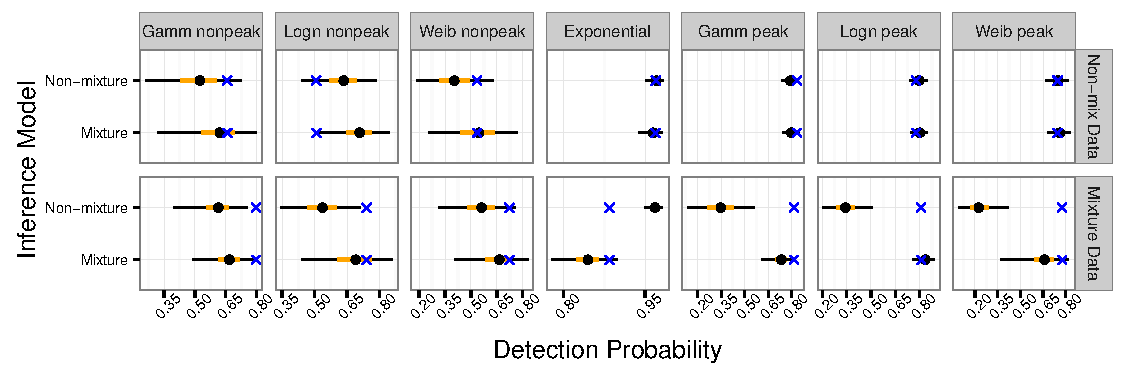
\includegraphics[width=0.98\textwidth]{Sims/SimFull/pdet_cater_correct.pdf}
\caption{\label{pdet_cater_correct} Sim 3 caterpillar plots of posterior 50\% and 95\% credible intervals for the marginal probability of detection $p^{(det)}$.  
Inference models come from the same family as the dataset but may differ in the presence/absence of a mixture component.  
Each column presents one family of simulated dataset.  
Upper plots show non-mixture datasets; lower plots show mixture datasets.  
`X' marks the expected marginal probability of detection based on true parameter values.}
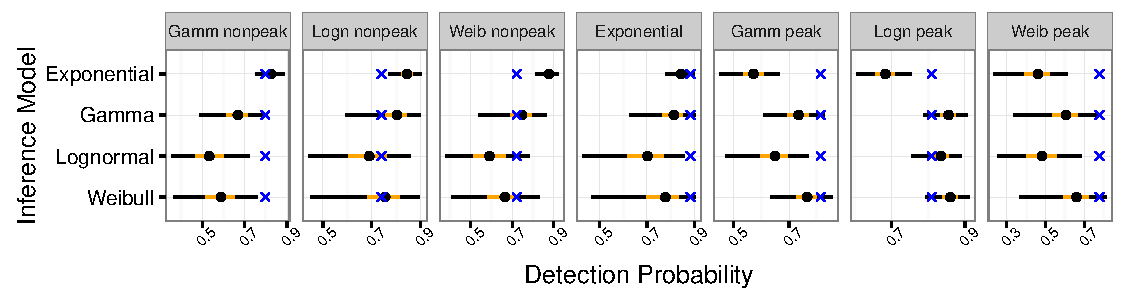
\includegraphics[width=0.98\textwidth]{Sims/SimFull/pdet_cater_family.pdf}
\caption{\label{pdet_cater_family}  Sim 3 caterpillar plots of posterior 50\% and 95\% credible intervals for the marginal probability of detection $p^{(det)}$. All data and inference models include mixtures.  
Each plot presents one simulated dataset.  
`X' marks the expected marginal probability of detection based on true parameter values.}
\end{figure}

As in Sim 2, for mixture exponential datasets only, mixture exponential inference models in Sim 3 returned accurate estimates of $p^{(det)}$ and had credible intervals from one-fourth to one-half as wide as from other inference models (Figure \ref{pdet_cater_family}).  
However, exponential mixture models were generally biased high for non-peaked datasets and low for peaked datasets.  
Lognormal mixture models tended to underestimate detection from non-lognormal datasets.  
Gamma models were more accurate than other models for non-peaked mixture datasets; gamma and Weibull both seem equally accurate for peaked mixture datasets.  
95\% credible intervals for gamma models were 15-35\% narrower than for both Weibull and lognormal models.

For every dataset we simulated, estimates of abundance covariate coefficients were virtually the same regardless of the TTDD employed.  
Estimates of detection parameters varied by context.  
In comparisons of mixture and non-mixture models within the same TTDD family (a la Sim 1), estimates were similar except when data derived from peaked mixture TTDDs.  
In that case, mixture models yielded narrower credible intervals than non-mixture models --- except in the exponential case, where non-mixture exponential models were overly precise.  
In comparisons of models across families (a la Sim 2), estimates across gamma, lognormal, and Weibull mixture inference models are always quite similar to one another.  
Credible intervals from exponential mixture models are wider for peaked data but narrower for exponential and non-peaked data.  


% The following plots of posteriors for abundance and detection parameters are just too large (and must be shrunk too small to make fit)
%\begin{figure}[h!]\centering
%\includegraphics[width=0.32\textwidth]{Sims/SimFull/Posteriors_select6.pdf}
%\includegraphics[width=0.32\textwidth]{Sims/SimFull/Posteriors_select2.pdf}
%\includegraphics[width=0.32\textwidth]{Sims/SimFull/Posteriors_select13.pdf}
%\end{figure}

\subsection{Model fit}\label{sec:modelfit}

Across all simulations, posterior predictive checks of by-interval counts provided only limited ability to identify poor model fits.  
For peaked and exponential mixture datasets (Sims 1 \& 3), posterior predictive checks clearly showed lack of fit for non-mixture inference models (Figure \ref{postpredmix}).  
For gamma, lognormal, and Weibull mixture datasets fit with an exponential inference model, second-interval posterior predictive values near to one often pointed a model misfit (Sims 2 \& 3).  
These are all cases where true data distribution has one more mode than the inference model can accommodate; in these cases, the second interval is hardest to fit, because of the mixture formulation of the models.  
For all other models, posterior predictive checks did not consistently indicate lack of fit.

\adam{I'm guessing I should not include the following: (1) my posterior predictive pvalues are not independent; (2) for instance, for the first interval, they stay very close to 0.5-0.6 --- the models are effective at getting the first interval right; (3) likewise, a post. p-value $>$ 0.8 during the 2nd interval likely shows model misfit; all of which raises the possibility that (4) multiple simulation under the null could provide a reference distribution of posterior p-values.}


\begin{figure}[h!]\centering
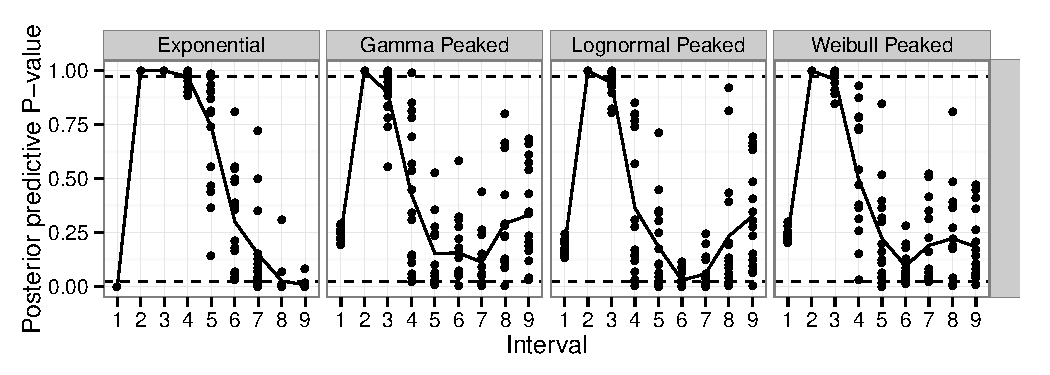
\includegraphics[width=0.78\textwidth]{Sims/SimZero/PostPredP_corr.pdf}
\caption{\label{postpredmix} Posterior predictive p-values by interval -- Pr$\left(p_{si}^{(rep)} > p_{si}\right)$ -- for peaked mixture datasets fit with non-mixture inference models of the correct TTDD family over 16 replicates (Sim 1).  
Trendlines show mean posterior predictive p-values.  
Dashed lines show central 95\% intervals.  
P-values near 0 or 1 potentially indicate poor model fit.}
\end{figure}

DIC showed a limited ability to select among models with different TTDDs.  
For peaked and exponential mixture datasets (Sims 1 \& 3), DIC regularly favored a mixture inference model over a non-mixture model (differences were always greater than 12).  
Also, when peaked gamma or lognormal mixtures were the true data model (Sim 2), DIC signalled against fitting an exponential mixture model (differences greater than 5).  
These are the same scenarios where posterior predictive checks highlighted model misfit.

DIC comparisons of TTDD family in the single replicate from Sim 3 were variable.  
For peaked mixture datasets, correct models were favored over mixture exponential inference models by at least 10 in gamma and lognormal cases and by 4 in the Weibull case.  
For the exponential mixture datasets, the exponential inference models was favored by at least 6 over all other models.  
For non-peaked mixture datasets, models were generally within 4 units of one another --- with the exception that the exponential mixture model was favored by 8 units for the lognormal mixture dataset.  
Considering that exponential models were biased for detection in non-peaked models (Figure \ref{pdet_cater_family}), we have little confidence in our DIC results for non-peaked models.  
DIC performance in Sim 3 may differ from Sims 1 \& 2 not only because of the addition of fixed and random effects, but also because DIC is calculated according to a different method.






\section{Results}\label{sec:results}

\section{Ovenbird analysis}

We fit mixture and non-mixture models from each family of TTDD to the Ovenbird dataset.  
Posterior predictive check p-values by interval (Table \ref{tbl:ovencounts}) show a clear lack of fit for the straight exponential model over the first three intervals.  
Two features of the data proved difficult to fit for all of the models: an increase in counts during the fourth interval, and a decrease during the final interval.  
Mixture models were better able to fit these features than non-mixture models.

\begin{table}[ht]
\centering
\begin{tabular}{lccccccccc}
  \hline
Minutes & 0-2 & 2-3 & 3-4 & 4-5 & 5-6 & 6-7 & 7-8 & 8-9 & 9-10 \\ 
Count & 596 & 69 & 62 & 68 & 43 & 33 & 35 & 27 & 14 \\ 
\hline
\multicolumn{10}{l}{Posterior predictive check $p$-values by model:}\\
\hline
Expo & 0.000 & 1.000 & 1.000 & 0.347 & 0.590 & 0.372 & 0.007 & 0.006 & 0.190 \\ 
  Gamma & 0.582 & 0.820 & 0.394 & 0.006 & 0.362 & 0.637 & 0.241 & 0.519 & 0.977 \\ 
  LogNormal & 0.571 & 0.943 & 0.471 & 0.005 & 0.322 & 0.554 & 0.165 & 0.407 & 0.974 \\ 
  Weibull & 0.582 & 0.862 & 0.401 & 0.005 & 0.359 & 0.616 & 0.221 & 0.509 & 0.982 \\ 
  Exponential Mix & 0.533 & 0.804 & 0.577 & 0.021 & 0.501 & 0.668 & 0.190 & 0.338 & 0.918 \\ 
  Gamma Mix & 0.593 & 0.720 & 0.431 & 0.015 & 0.439 & 0.670 & 0.246 & 0.476 & 0.947 \\ 
  LogNormal Mix & 0.576 & 0.806 & 0.508 & 0.016 & 0.421 & 0.627 & 0.197 & 0.413 & 0.951 \\ 
  Weibull Mix & 0.596 & 0.734 & 0.411 & 0.013 & 0.421 & 0.663 & 0.252 & 0.492 & 0.958 \\ 
   \hline
\end{tabular}
\caption{\label{tbl:ovencounts} Ovenbird counts and posterior predictive check p-values by observation interval for each model across all surveys.}
\end{table}

Ovenbird results reflect several patterns that were observed in the simulation studies for both exponential and non-peaked data.  
Figure \ref{ovenposteriors} presents caterpillar plots of posterior estimates for model parameters, overall detection probability $p^{(det)}$, and the log10 number of Ovenbirds uncounted.  
Shape parameter estimates from mixture models favor non-peaked distributions --- i.e., detection rates are higher earlier in the observation period --- however, in mixture gamma and Weibull models, an exponential TTDD model ($\alpha=1$ or $k=1$) is well within 95\% credible intervals.  
These pattern is similar to our simulations involving non-peaked mixture datasets, especially exponential and lognormal.

Abundance covariate coefficient estimates are virtually the same for all TTDD models.  
Detection parameter estimates are similar by mixture type across gamma, Weibull, and lognormal TTDD models.  
Credible intervals from exponential mixture models are more precise than for non-exponential mixture models.  
Within mixture type, estimates of detection probability across all surveys, $p^{(det)}$, are lower and much more uncertain for gamma, Weibull, and lognormal models than for exponential.

DIC calculations prefer the exponential mixture TTDD to the lognormal, Weibull, and gamma mixtures (differences of 6.95, 10.7, and 11.5, respectively), and these differences closely mirror those from the exponential mixture dataset in Sim 3.  
However, Sim 3 demonstrated that DIC for non-peaked mixture data may not be reliable; indeed, for the simulated non-peak lognormal mixture dataset, the exponential mixture TTDD was favored by over a 4-unit difference; yet, its posterior 95\% credible interval for detection probability did not contained the true value, while it was within a central 60\% credible interval for all three other mixture models.  
In short, DIC may not be trustworthy in this situation.

Credible intervals for two of the abundance parameters do not contain zero, thereby suggesting notable effects.  
Select- and partial-cut logging events of the 1990s depressed local Ovenbird abundance during the study perior to roughly 25-50\% of the abundance for unlogged sites.  
Credible intervals for Site Age indicate that each decade of age increases abundance from 1.5-13\%.

\begin{figure}[h!]
\includegraphics[width=0.98\textwidth]{OVEN/oven_sum/OVEN_posteriors.pdf}
\caption{\label{ovenposteriors} Caterpillar plots of posterior parameter estimates for models fit to the Ovenbird data.  
Abundance and detection parameters are identified by (A) and (D), respectively.  
Gamma is the mixing parameter.  
Alpha, k, and sigma\_det are shape parameters for gamma, Weibull, and lognormal distributions, respectively.  
p\_det and log10(Uncounted) are the detection probabilty and the number of birds present but not counted across all surveys.  
Black bars are 95\% credible intervals, orange bars are 50\% credible intervals, and black dots are posterior medians.}
\end{figure}






\section{Discussion}

Historically, analysis of removal-sampled data assumes constant detection rates throughout the sampling period.  
This assumption provides an intuitive null model and is analytically tractable.  
However, although analysis of removal models has grown more sophisticated in recent years, the constant-detection assumption nonetheless continues unquestioned.  
In our study, we have formulated a model for non-constant detection patterns using a time-to-event approach within a hierarchical N-mixture framework.  
Our results demonstrate that, for better or worse, the assumption of constant detection is a very strong assumption.  
When it is correct, it is the most accurate and precise of TTDD models, but when detection rates are not constant, it results in significant bias.  
Models with non-constant TTDDs, on the other hand, can adapt to a wider variety of detection patterns.

We modeled two varieties of heterogeneous detection in conjunction with one other: (i) time-varying detection rates, as modeled by non-exponential TTDDs, and (ii) detection heterogeneity among subgroups of individuals, as modeled by mixture TTDDs.  
The exponential TTDD, even when modeled with a mixture component, results in biased estimates of detection when detection actually varies with time.  
Gamma, Weibull, and lognormal TTDDs, with their extra parameter, are more accurate in handling non-constant detection data, though they are less precise when estimating data with constant detection.

The utility of applying a mixture TTDD for constant-detection models has been identified several times \citep{Pledger2000, Farnsworth2002, Alldredge2007, Reidy2011}.  
The mixture allows an analysis to account for detection heterogeneity across easy- and hard-to-detect subgroups of a population.  
Even so, some recent studies have assumed the absence of a mixture \citep{Solymos2013, Amundson2014}.  
Our study indicates that mixtures are useful even when a non-constant TTDD is used for hard-to-detect individuals.  
Models that include a mixture generally perform well even when no heterogeneity is present, but models that omit a mixture are biased and overly certain when detection heterogeneity exists.  
Indeed, for peaked datasets, mixture models can outperform non-mixture models even in the absence of heterogeneity.

In a limited set of situations, posterior predictive checks and DIC can identify when non-mixture or exponential TTDDs inadequately describe the marginal pattern of detections over time.  
But in many situations, neither tool points a clear way to select the correct family of TTDD.  
Given the bias that can result from assuming constant detection or omitting a mixture component, conservatism dictates that non-constant TTDDs with a mixture should be preferred.  
Among the TTDDs we considered, the mixture gamma TTDD appears to provide the best combination of accuracy and precision for non-peaked data.  
For peaked data, gamma and Weibull models seem about equally as good.  
MCMC sampling from gamma models required from 5-10 the run time as lognormal and Weibull models.

If the estimation of effect parameters is the primary interest, then our results suggest that the exact choice of TTDD may not be important.  
Abundance effect estimates are similar regardless of the chosen TTDD, while detection effect estimates are similar for all mixture non-exponential TTDDs.  
These finding may well not hold if the same covariate is modeled in both abundance and detection models \citep{Kery2008}.

Because our focus is detection, we assumed Poisson-distributed abundance for simplicity.  
Abundance distributions that have been used to account for overdispersion include negative binomial, zero-inflated Poisson, and Poisson with survey-level random effects.  
The pattern of counts in our Ovenbird data actually reflect underdispersion, so a Conway-Maxwell Poisson distribution, which can model both overdispersion and underdispersion, may be more appropriate \citep{Wu2015}\adam{apparently, Sellers et al. (in Wu) has a comprehensive overview of the CMP.}

% Overview: Wu15
% ZIP: Etterson, Solymos12
% NB: Royle04(?)


At present, Stan does not sample discrete parameters, so the ability to marginalize out the discrete-valued latent variables $N_{s}$, as we did, can greatly facilitate MCMC sampling.

% \adam{I have contemplated on and off including a discussion of broad priors and the limit behavior as $\varphi \to 0$, but I think it's not really on topic.  
% Note: now that I've seen van Dishoeck and Manntyniemi, perhaps I should worry about informativeness in priors.}

% All estimates are based on extrapolation of the observed detections\\
% -- a) explore the tail more?  I think that'd require a lot of data\\
% -- b) requires extended observation periods or full detection data (Alldredge?)\\
% same goes for sample size

% Really, I have totally ignored the discussion of the true value of p, which I have tended to simulate in a fairly high range


To improve our choice of TTDD and/or its parameters, it makes sense to obtain more data in one of a few ways.  
One approach is to collect complete detection history records, not just first time-to-detection observations \citep{Alldredge2007}.  
This may not be feasible in studies like MNFB, where many species are observed.  
Another approach is to conduct a longer survey that better assesses the tail distribution of the TTDD; however, the longer the survey is, the greater the risk that individuals enter/depart the study area or are double-counted, which violates removal sampling assumptions \citep{LeeMarsden2008, Reidy2011}.  
A third idea is to obtain more precise time-to-detection data, even exact time-to-detection data.  
In some early explorations of our model considering just an exponential mixture TTDD, we found that credible intervals for Ovenbird detection probability were 20-25\% narrower using 9-interval surveys compared to more traditional 3-interval surveys (0-3, 3-5, and 5-10 minutes).  
For all of the above, a small pilot study may be a practical starting point.  


With the increasing use of microphone arrays for automated detection \adam{refs}, it is tempting to think TTDD models may be valuable for microphone-collected data.  
This should be the case when variations in detection result solely from organismal behaviors, such as bout singing, or if we wish to model individual random effects in the detection model.  
However, some explanations for non-constant detection are explicitly related to the observation process --- either effects of the observer on animal behavior or variations in observer effort caused by survey methodology.  
The assumption of constant detection seems more plausible in studies where observers are absent, though detection heterogeneity may still exist across subgroups of the population.

Application of TTDD modeling within the N-mixture framework should be straight-forward for other time-to-detection datasets, such as full detection-history and double-observer.  
The key difference will be in the data model, in that responses will take a different form than multinomially distributed first times to detection.  
But the underlying abundance and detection models remain the same.  
\adam{Time-heterogeneous models have been done for mark-recapture (Farcomeni and Scacciatelli 2013, who reference Hwang and Chao 2002).}

The time-to-detection approach in our model is a departure from the probability-of-detection approach that has been used in distance-removal modeling \citep{Farnsworth2005, Diefenbach2007, Solymos2013, Amundson2014}\adam{Alldredge2007?}.  
In a distance-sampling context, the probability of detection for any individual is framed as the joint probability of two independent detection events: (i) availability for detection, which occurs during an observation period with probability $P_a$, and (ii) detection of the available individual by an observer, $P_b$, also known as perceptibility \citep{Williams2002, Kery2008, Nichols2009}\adam{I haven't read Williams2002 -- cited in Royle2004.  
I'm  beginning to think this may have too-numerous antecedents to cite... in Reidy, the earliest reference is Marsh and Sinclair 1989.  
See also McCallum 2005.}.  
In avian point-counts, because the overwhelming majority of detections are auditory, $P_a$ is understood to be the probability that a bird vocalizes during the observation period.  
Meanwhile, perceptibility is treated as a function of distance $d$: $P_b = g(d)$, with nearby available individuals being detected with higher probability than distant individuals.  
The probability of detection is thus formulated as availability times perceptibility: $p^{(det)} = P_aP_b$.  
Multiple studies have demonstrated that failure to incorporate distance leads to systemic bias in estimates of abundance \citep{EffordDawson2009, Solymos2013}.

The time-to-detection model as presented here in our study does not incorporate distance.  
Consequently, our definition of a TTDD necessarily represents an averaging across distance classes and a consequent loss of information if distance data are available.  
We can modify our model to account for distance.  
To be consistent with earlier distance-removal studies \citep{Farnsworth2005, Amundson2014}, we could: (i) define a time-to-\textit{availability} distribution $F_T^A(t)$ in the same manner that we have defined a TTDD in this study, (ii) modify Equation \ref{eq:pdet} to reflect the detection distance to individual $q$: $p_{sq}^{(det)} = g(d_q) F_T^A(C_I|\textbf{X}_{s}^D, \textbf{Z}_{s}^D, \boldsymbol{\theta})$, and (iii) tweak our data model accordingly.

However, our analysis makes possible a different strategy that is more consistent with a time-to-event conceptualization of the problem.  
Rather than define availability and perceptibility as independent detection events over the course of the observation period, we can define them at the event level.  
In terms of the model we have presented in this paper, this is equivalent to redefining the time-to-detection hazard function, $h_{sq}(t)$ --- which is now a function of the distance to individual $q$ --- as the product of the time-to-availability hazard function $h_{s}^A(t)$ and the perceptibility function $g(d/`8-_q)$.  
So, $h_{sq}(t) = g(d_q) h_{s}^A(t)$.  
From standard survival analysis results, $p_{sq}^{(det)} = 1 - \exp\left(-g(d_q)\int\limits_0^{C_I} h_{s}^A(u)du\right) = 1 - \left[1 - F_T^A(C_I|\textbf{X}_{s}^D, \textbf{Z}_{s}^D, \boldsymbol{\theta}) \right]^{g(d_q)}$.

In short, the time-to-event conceptualization frames perceptibility as a rate-of-availability multiplier rather than as a probability-of-availability multiplier.  
In a context where rates of availability are allowed to vary from individual to individual, this makes an intuitive sense --- a bird that sings twenty times during the observation period should have its overall detection probability discounted much less than a bird at the same distance which only sings once.  
This is an area of ongoing exploration.


% Skeptics of removal sampling: Johnson08, EffordDawson09, Reidy11

%\subsection{Lit Notes on Distance and Poisson Abundance}
%--- Borchers is all about this\\
%--- Farnsworth2005, EffordDawson2009, Amundson2014\\
%----- particularly noticeable with finite mixture models\\
%- Oedekoven2013 is all about covariates on distance sampling curve\\
%- necessity of using distance, too, is backed by Solymos2013, (Buckland et al 2001, 2004), Farnsworth2005, EffordDawson2009...\\
%
%Poisson assumption (do I want to discuss underdispersion?\\
%--- Denes et al 2015 discuss how Poisson assumption leads to bias in the absence of detection heterog (ref to Solymos et al 2012) or when inflated zeros are present (Joseph et al 2009) [with the obvious remedies being: NegBin and ZIP, respectively]... but is that negated by our underdispersion?\\
%
%`Unmodeled individual heterogeneity causes population size to be underestimated using capture-recapture and removal methods' (from Efford and Dawson, who cite Otis et al. 1978)\\


% Ideas for the future
% (i) Distance-removal time-to-event model
% (ii) Fit more species from this dataset over full survey duration; maybe some model selection (even Bayesian)
% (iii) Take a stab at modeling habitat
% (iv) Model for non-independent singing?
% (v) Model for density-dependent singing? (only valid, I think, if we have lots of underdispersion from(ii))
% (vi) I know I've  been warned off it, but automated detection intrigues me
% (vii) Further testing of existing model: sensitivity to priors, performance for varying detectability levels, sample size, # intervals
% (viii) Incorporate spatial random effects.  
This work has already been done, just not for TTDD models, but the real spatial dependency should be in abundance, not detection
% (ix) Comparison of methods -- just looking at my lit review, there are gadzooks strategies that people have proposed.  
Combining/comparing them seems maybe informative?  To what degree has this already been done?

\bibliography{masterbib}
\bibliographystyle{biom}



\end{document}
